%% ID: superball
%% TITLE: Superball
%% TYPE: question
%% QUESTIONTYPE: numeric
%% CONCEPTS: energy, momentum, momentumii
%% VIDEOS: 
%% LEVEL: 6
%% TOPIC: mechanics/dynamics
%% ORDER: 9

\begin{problem}[Superball] 
{\exposition{A basketball of mass \vari{m_1} and radius  \vari{r_1} and a tennis ball of  mass \vari{m_2} and radius \vari{r_2} are held with the bottom of the tennis ball touching the top of the basketball, and the bottom of the basketball is a height \vari{h} above the ground. The balls are then dropped together.} \question{What is the maximum height that the centre of mass the tennis ball reaches after the balls bounce off the floor?}

Assume that the mass of the tennis ball is much smaller than the mass of the basketball, and that all collisions are elastic.}
{\stress{Found in Harvard questions of the week, but also seen in many different places}}
{Initially, the acceleration of both balls is the same and is equal to \vari{g}. Both balls fall a distance \vari{h}, and by using the equation of motion \valuedef{v^2}{u^2 + 2ax}{} we find that they both have a speed \valuedef{v}{\sqrt{2gh}}{}. The balls bouncing off the ground can be treated as two subsequent collisions. When the basketball hits the ground, as the mass of the Earth is so much greater than that of the basketball that very little kinetic energy is transferred to it, and as the collision is elastic the result is that the basketball ends up moving upwards with speed \vari{v}.

\begin{figure}[h]
\centering
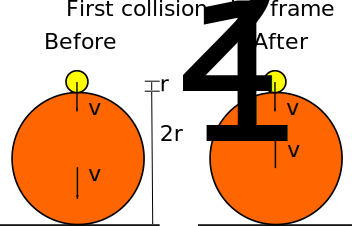
\includegraphics[width=1.0\textwidth]{../../../figures/dynamics_tennis_basket_ball_first.svg}
\caption{}\label{fig:dynamics_tennis_basket_first}
\end{figure}

The second collision occurs with the basketball and tennis ball moving towards each other, each travelling at a speed \vari{v}. As the basketball has a much higher mass, the frame of reference of the basketball is almost exactly the zero momentum frame, and in this frame the tennis ball starts off with a speed \vari{2v} moving towards the basketball, and after the collision has a speed of \vari{2v} away from the basketball. In the frame of reference of the Earth, the tennis ball therefore has a final speed \vari{3v} upwards.

\begin{figure}[h]
\centering
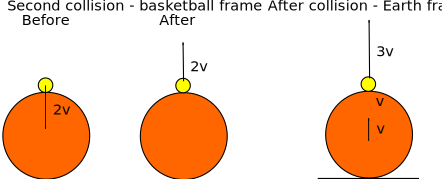
\includegraphics[width=1.0\textwidth]{../../../figures/dynamics_tennis_basket_ball_second.svg}
\caption{}\label{fig:dynamics_tennis_basket_second}
\end{figure}


By conservation of energy, the tennis ball will gain a height \valuedef{\Delta H}{\frac{(3v)^2}{2g}}{}, and since \valuedef{v}{\sqrt{2gh}}{}, this gives \valuedef{\Delta H}{9h}{}. The centre of mass of the tennis ball was at a height \vari{2r_1 + r_2} before the ball bounced, and therefore the final height of the centre of mass will be given by \valuedef{H}{9h + 2r_1 + r_2}{}.

\answer{The tennis ball bounces up a height \valuedef{\Delta H}{9h}{}, and so the final height of the centre of mass will be given by \valuedef{H}{9h + 2r_1 + r_2}{}.}
}
\end{problem}